% This is an LPSC Abstract template for LaTeX 2e that is based off of the
% LaTeX article document class.

% $Id: lpsc_abstract.tex 11 2008-01-31 15:42:07Z rbeyer $

% Copyright (C) 2005,2007 Ross A. Beyer
% Copyright (C) 2008 Ross A. Beyer and Moses P. Milazzo
% Copyright (C) 2014 Moses P. Milazzo
%
% This work is licensed under the Creative Commons
% Attribution-Noncommercial-Share Alike 3.0 License. To view a copy
% of this license, visit http://creativecommons.org/licenses/by-nc-sa/3.0/;
% or, (b) send a letter to Creative Commons, 171 2nd Street, Suite
% 300, San Francisco, California, 94105, USA.

% Use the LaTeX article class.  Pass any options you like to article, except
% twocolumn.  We take care of that in the lpscabs pacakage below.
\documentclass[twoside, 10pt]{article} 

\usepackage{times}		% Nice fonts, optional
\usepackage{url}                % Needed for wrapping long URLs
\usepackage[pdftex,colorlinks=true,urlcolor=blue,citecolor=black,linkcolor=black]{hyperref}
								% Puts actual hyperlinks in your PDF, optional.
								
\usepackage{graphicx}			% Nice graphics, optional

\usepackage[numbers]{natbib}	% Nice references, optional
% These commands are relevant to natbib.  If you don't use
% natbib for your references, you should get rid of these, as well.
\renewcommand{\bibfont}{\small}	% Change the font size of the bibliography
\setlength{\bibsep}{0pt}		% Remove the spacing between bib entries


\usepackage{paralist}			% For compressing bibliography into a paragraph

\usepackage{balance}			% For balancing columns on the page. Note that to use this, you must also uncomment the balance command below.

\usepackage{lpscabs}			% This is to take care of some LPSC abstract
								% document-specific things and set sizes.					

\usepackage[super]{nth}			% This provides simple commands to deal with superscripts on numbers. Totally optional.

\usepackage{paralist}			% For compressing bibliography into a paragraph; Required if using the \parabib bibliography command

\usepackage{balance}			% For balancing columns on the page.



% To compress the section titles even more, use the titlesec package.
\usepackage[tiny,compact]{titlesec}

\titlespacing*{\section} {0.20in}{1.5ex plus .5ex minus .2ex}{1.3ex plus .2ex} % This indents the section titles by 0.0in and defines the 
        														% spacing above and below the sections. If you want 
														% deeper indentation, increase the value of the first argument.
														% If you want different vertical spacing, muck with the second
														% argument. The third defines the relationship between the
														% section titles and the paragraph that comes after.
																	
\setlength{\bibmarginindent}{0.2in}	% This sets the indentation level of the itemization of the bibliography items if the \biblist 
							% bibliography option is used for the bibliography. Otherwise it's ignored. At 0.2in, the items
							% line up with the column margins.


\begin{document}

% The \titlearea command takes two arguments in curly braces {}.  The first
% will be used as the title, and the second as the author info.


\titlearea{Using \LaTeX\ to write an LPSC Abstract.}{Ross A. Beyer$^{1,2}$ and Moses P. Milazzo$^{3}$, $^1$Carl Sagan Center at the SETI Institute, $^2$NASA Ames Research Center, MS 245--3, Moffett Field, CA, USA (\href{mailto:Ross.A.Beyer@nasa.gov}{Ross.A.Beyer@nasa.gov}), and $^3$Astrogeology Science Center, United States Geological Survey (\href{mailto:moses@usgs.gov}{moses@usgs.gov})}

% Here is an example with just one author:
%
%\titlearea{Using \LaTeX\ to write an LPSC Abstract.}{Ross A. Beyer, NASA Ames Research Center, MS 245-3, Moffett Field, CA, USA (Ross.A.Beyer@nasa.gov)}

% Here is an example with more than one author from more than one place:
%
% \titlearea{Using \LaTeX\ to write an LPSC Abstract.}{Ross A. Beyer$^{1,2}$, John Q. Public$^{a}$, and Jane Doe$^{\dag}$, $^1$Carl Sagan Center at the SETI Institute, $^2$NASA Ames Research Center, MS 245-3, Moffett Field, CA, USA (Ross.A.Beyer@nasa.gov), $^{a}$123 Sesame Street, New York NY, USA, $^{\dag}$890 Somewhere, ID, USA}

% Uncomment \usepackage{balance} above to use this:
\balance{}

\vspace{4cm}
\section*{Introduction}
There used to be a \LaTeX\ template and a style file for writing
Lunar and Planetary Science Conference (LPSC) abstracts available
on the LPSC Web site.  However, no such template has been available
for some time, and we found ourselves dragging the old one out.  It
was full of scary \TeX\ commands and had a date from 1996 in it,
so we decided to start from scratch and write a
\href{https://github.com/MosesAstro/LaTeX_Templates/tree/master/LPSCAbstractLaTeXTemplate}{template} based
on \LaTeX's own article class and a short \LaTeXe\ package file.
Most of the \LaTeX\ work is based on~\cite{kopka2003guide}. Fortunately, the 
requirements for LPI-sponsored meeting abstracts (like LPSC)
are reasonably relaxed \citep{LPSC}.

\section*{Title area:}

The title mechanism for this template is a simple command,
\verb=\titlearea=, which takes two arguments, the title text and the
author info text. We have commented out a few multiple author styles above,
near the \verb=\titlearea= section of this source file. Choose the
one that works for you. The title text is made using {\sc Smallcaps} similarly to the LPI Word
template.  If you would like a different style, it should be easy to go in to 
the \texttt{lpscabs.sty} file and change it.

\section*{Section styles:}

In general, people try to put lots of information into their LPSC
abstracts, and want to minimize the space being taken up by section
headers.  You could redefine the sectioning commands to change their
styling if you like, or you could just use this package's customized 
\verb=\section= command (as we have done in this example).  
You can also use the \texttt{titlesec} package with the \texttt{small} 
and \texttt{compact} options to further compress the font size and 
space around titles.

\section*{Figures:}

\begin{figure}[b]
\begin{center}
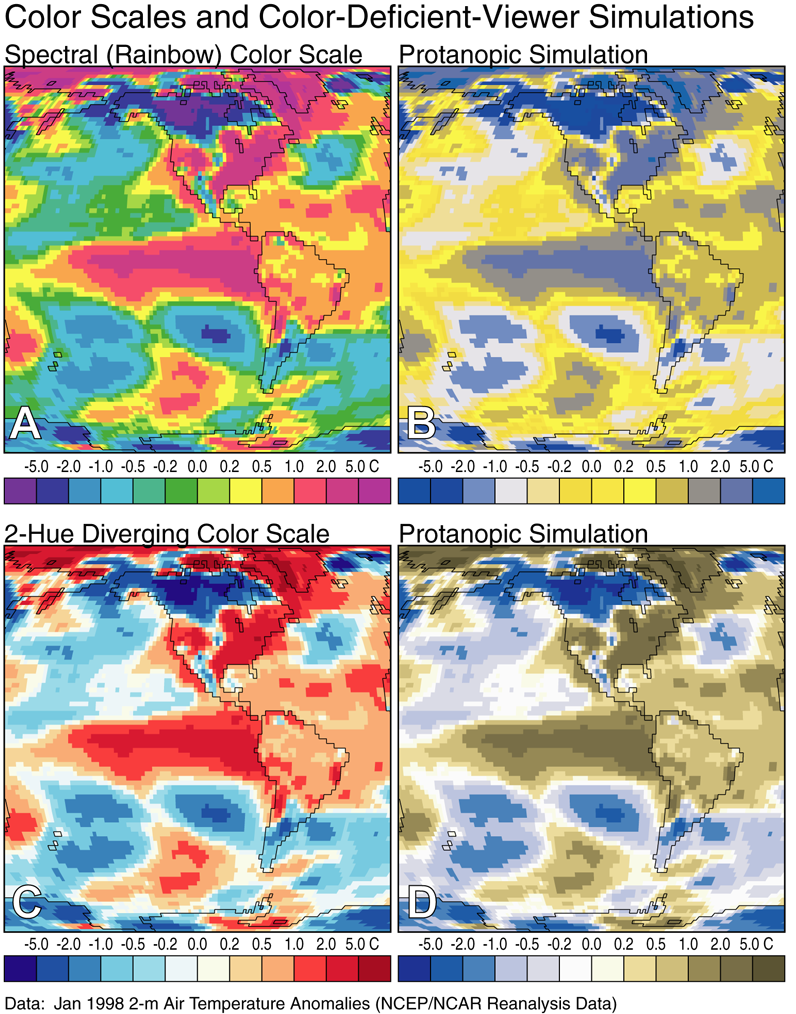
\includegraphics[width=\columnwidth]{lb_fig1.png}
\caption[Color Scales and Color-Deficient-Viewer Simulations]{\label{color_scales}
    This is Figure~1 from~\cite{light2004end}.}
\end{center}
\end{figure}

Good figures are hard to make, there's no question about it.  That
goes double for deciding which figures to include in your 
space-limited abstract.

When you make the decision to create a color figure, take some time
to think about the colors that you use.  We think that a  strong case has 
been made~\citep{light2004end,borland2007rainbow} for not using the
typical rainbow-spectrum color scheme (e.g. Fig.~\ref{color_scales}).
Just because you decide to use color doesn't mean that you need to
use \emph{all} of the colors.  Don't confuse ``pretty'' with
``meaningful.''

In addition, \citep{green2011colour} suggests that color schemes
should be perceived as monotonically increasing (or decreasing)
when used to display intensity maps (such as
topography, temperature, etc.). This is not usually possible with 
most rainbow color schemes. A monotonically increasing color scheme 
is also correct whether printed in color or grayscale (e.g., Fig~\ref{SaturationColors}).

If you need figures or tables to be the full width of the page,
just use their starred versions, like \verb=\begin{figure*}= instead
of \verb=\begin{figure}=.  If you have problems with double-column-wide
floats, you may need to monkey with the \verb=\dbltopfraction=
setting or other style parameters for floats (either in the
\texttt{lpscabs.sty} file or simply via
\verb=\renewcommand{\dbltopfraction}{}= in your abstract \texttt{.tex}
file).

\begin{figure*}
\begin{center}
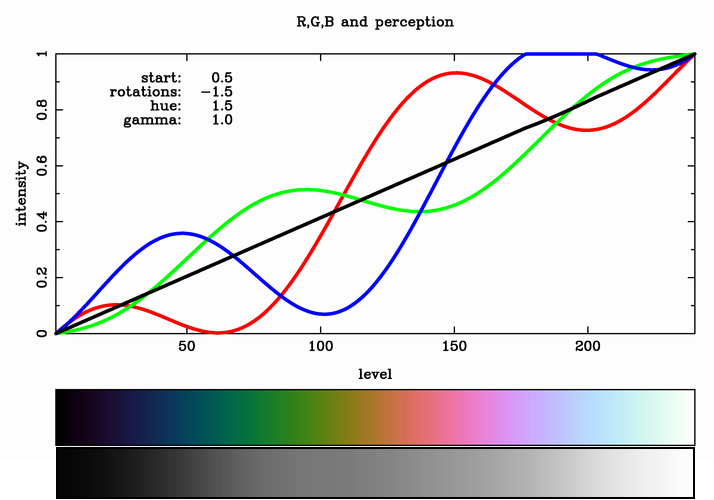
\includegraphics[width=0.825\textwidth]{rgb-grey-morehue.png}
\caption[CubeHelix Color Schemes]{
\label{SaturationColors}
    Modified from \href{https://www.mrao.cam.ac.uk/~dag/CUBEHELIX}{https://www.mrao.cam.ac.uk/~dag/CUBEHELIX}.
    The color and greyscale bars are both increasining in brightness monotonically.
    }
\end{center}
\end{figure*}

\section*{URLs and hyperlinks:}

The odds are good that most people will read this
abstract on computer screens via a PDF reader rather than
on paper.  PDFs can contain active hyperlinks that can start a
Web browser or an email client. The
\verb=hyperref= package helps you do this.  It is used in this
example file, and there are blue links that you can click on in
this document.

The \verb=hyperref= package has some options that we should probably 
detail.  Here's a copy of the command in this document (new lines
are for clarity):
\begin{verbatim}
\usepackage[pdftex,colorlinks=true,
  urlcolor=blue,citecolor=black,
  linkcolor=black]{hyperref}
\end{verbatim}
\noindent
The options in the square brackets are important, and
\href{http://www.tug.org/applications/hyperref/manual.html}{http://www.tug.org/applications/hyperref/manual.html} details
all of them.  The first item \verb=pdftex= is because we mostly use
\verb=pdflatex= to create PDF files from our \verb=.tex= files; you may 
need a different option here.  You may wonder
why we set \verb=citecolor= and \verb=linkcolor= to black.  The
\verb=hyperref= package is good, it creates links for many 
things in the document, and gives them unique colors.
However, in this short document, that's visually distracting. 
The links are there, they're just black. You can click on the references
numbers, like this one:~\citep{kopka2003guide} (which won't do much since
the references are on this page), or figure numbers like
this:~\ref{color_scales}.


\section*{Copyright Information:}

This work is licensed under the Creative Commons
Attribution-Noncommercial-Share Alike License. To view a copy
of this license, visit \href{https://creativecommons.org/licenses/by-nc-sa/4.0/}{https://creativecommons.org/licenses/by-nc-sa/4.0/}

Does this mean that if you write an abstract using this template that
you are required to credit us and to release the paper under
the same kind of Creative Commons license?  Nope. What it does do is allow
anyone, even the LPI Meeting Staff, to take a copy of this template
and modify it (or not), and place it on their web pages for folks
to use.

Why not just dedicate it to the public domain?  Well,
we did spend some time on it and would like to be recognized.  Using
the Creative Commons license above allows us to retain copyright,
request that derivative templates credit us, but also allow for
\emph{anyone} to make derivative works, in addition to a few other
rights and restrictions.  If you want to know more, visit the
Creative Commons web site at \href{https://creativecommons.org/science/}{http://creativecommons.org/science}.


\section*{Works that you reference:}

Using \texttt{natbib} with the \texttt{numbers} option and the included
\texttt{lpsc} bibliographystyle approximates the reference-style
that has emerged for LPSC abstracts over the years \citep{LPSC}. 
 We have included two helper commands to achieve a 
close approximation to the LPI template bibliography style.
\verb=\parabib= is designed to use as little space as possible; it fits all 
of the references into a single paragraph. \verb=\listbib= is designed to 
provide a cleaner-looking, but less space-efficient bibliography.


% Use \parabib if you want to have all references in a single paragraph.
\parabib{templatebibliography}{lpsc}

% If, instead, you want each of your references on a separate line, use \listbib.
%\listbib{/Volumes/Work/Documents/LaTeX/Bibliography/bibliography}{lpsc}{\bibmarginindent}

\end{document}
